\newpage
\section{Resultados}

\subsection{Onda de saída}

A onda de saída obtida para o oscilador a cristal é mostrada na figura \ref{f_saida}, onde a frequência do sinal é de 10.01088MHz. A figura de Lissajous está na figura \ref{f_lissajous}.


\begin{figure}[H]
	\centering
	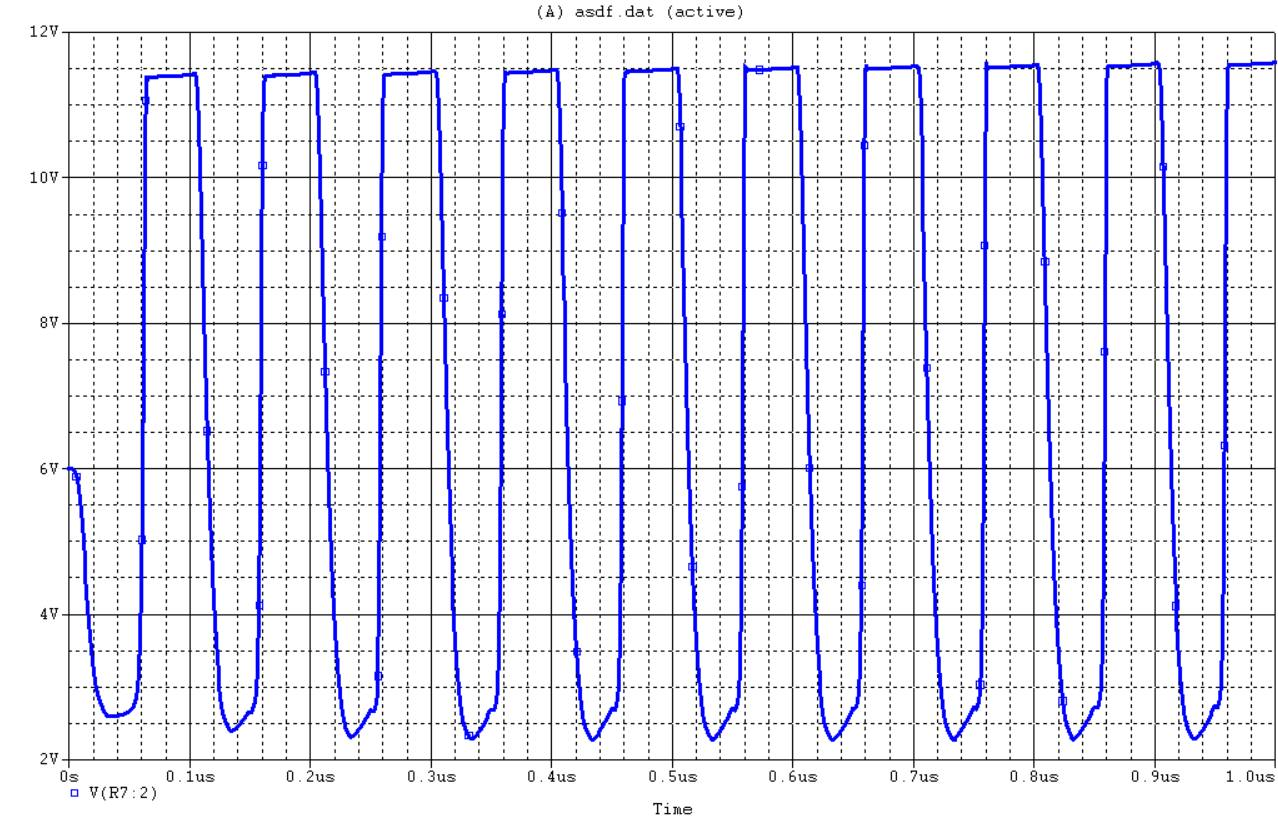
\includegraphics[scale=0.3]{Imagens/saida.jpg}
	\caption{Onda de saída para o oscilador a cristal.}
	\label{f_saida}
\end{figure}

\begin{figure}[H]
	\centering
	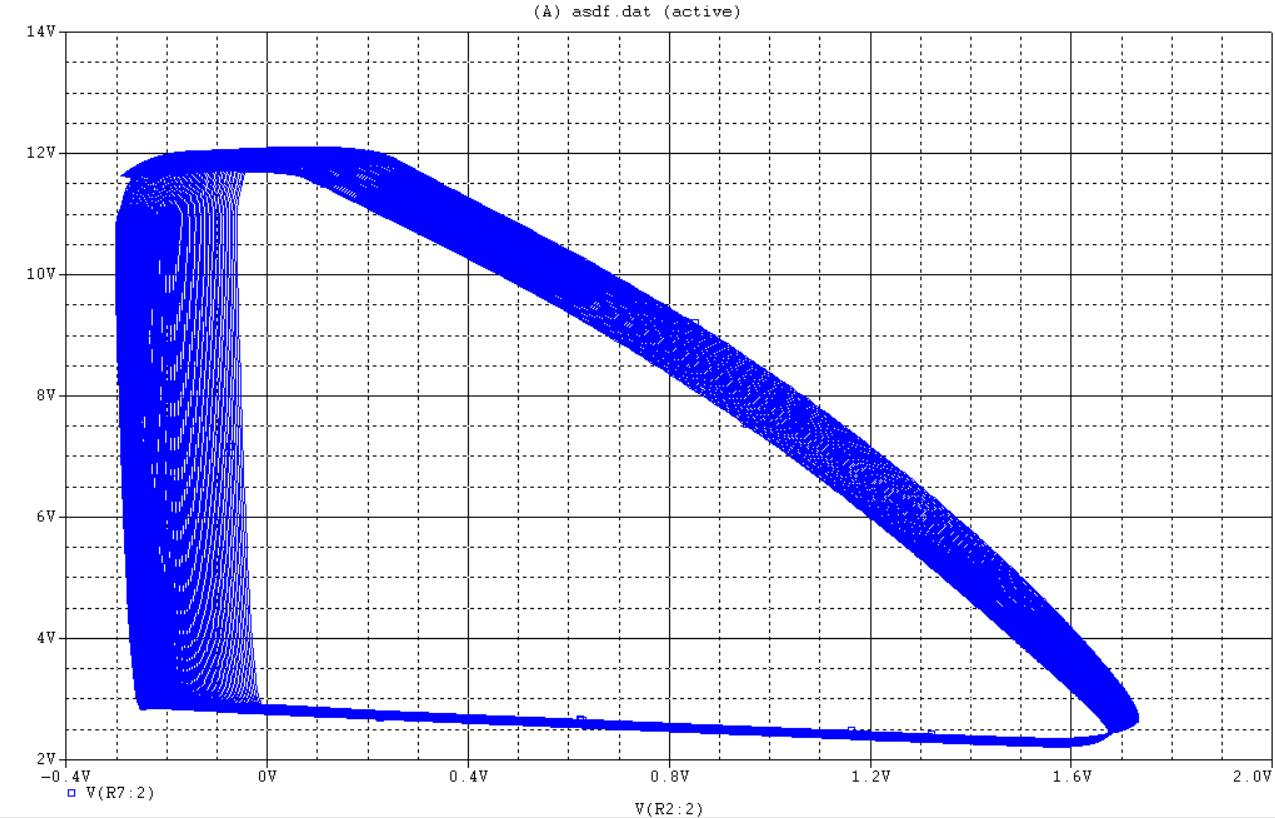
\includegraphics[scale=0.3]{Imagens/lissajous.jpg}
	\caption{Figura de lissajous.}
	\label{f_lissajous}
\end{figure}


\subsection{Influeência da ponta de prova}
Após colocar a ponta de prova do osciloscópio, a frequência alterou para 10.01155MHz, mostrando que há uma pequena interferência no periodo do oscilador.

\subsection{Variação da tensão de saída e critério de estabilidade}

A tabela \ref{t_estabilidade} mostra os dados obtidos variando-se a tensão.

\begin{small}
	\begin{table}[H]
		\begin{center}
			\caption{Frequência de oscilação obtida variando-se a tensão de circuito}
			\begin{tabular}{l|l}
				\hline
				Tensão de & Frequência [MHz] \\
				entrada [V]&  \\
				\hline
				9.6 & 10.01071 \\
				\hline
				12.0 & 10.01088 \\
				\hline
				14.4 & 10.01119 \\
				\hline
			\end{tabular}
			\label{t_estabilidade}
		\end{center}
	\end{table}
\end{small}

A estabilidade relativa obtida foi de 47,948 [ppm].

